\thesischapterexordium

\section{研究工作的背景与意义}

在很多研究领域,研究进展的取得往往需要依赖大量数据的分析。 比如在天体物理学领域, 为了给黑洞“照相”, Bouman等人需要处理5PB的数据\citing{akiyama2019first}。在生物医学领域, 一个人体样本的基因组数据会超过 100GB,由于一次实验会收集成百上千的人的数据,因此数据量十分巨大\citing{宁康2015生物医学大数据的现状与展望}。此外,由于记录数据的设备越来越多其他领域数据量也在不断扩大,比如传感器记录的行动数据、基因数据、照片、语音、金融日志、网络数据等。

海量数据被冠以术语Big Data, Big Data 至少包含3层含义\citing{beyer2012importance},即数据量大(Volume of data)、 数据处理速度快(Velocity of processing the data)与数据多样 (Variety of data),合称“3V”。对于这样的数据往往需要使用一些自动化的方法来分析数据中重要的模式和子结构或者对数据进行压缩,这些方法包括聚类和降维。粗略地说,前者即是将数据分为不同的类,使得同类的数据相似,不同类的数据不相似,后者是将数据投影到一个低维空间使得高维空间的数据的结构能够在低维尽可能保留。对于聚类经典的方法有$k$-means\citing{macqueen1967some}、 Spectral Clustering\citing{von2007tutorial}等,经典降维方法有PCA\citing{pearson1901liii}、 ISOMAP\citing{tenenbaum2000global}、 LLE\citing{roweis2000nonlinear}等。

与此同时,伴随信息技术的发展,人与人的链接变得日益密切,相关的文本、图像、音频等数据不断增加形成了大数据。为帮助人们从这些数据中梳理出有价值的信息,数据挖掘(Data Mining)技术应运而生。所谓数据挖掘便是从大量无序的数据中发现隐含的、有效的、有价值的、可理解的模式, 进而发现有用的知识,并得出时间的趋向和关联, 为用户提供问题求解层次的决策支持能力\citing{贺玲2007数据挖掘中的聚类算法综述}。在这些背景下,聚类作为一种主要的数据挖掘手段收到人们的重视,得到了蓬勃的发展。

故本篇文章聚焦聚类问题\citing{孙吉贵2008聚类算法研究,贺玲2007数据挖掘中的聚类算法综述,周涛2012数据挖掘中聚类算法研究进展}。这里给出Everitt\citing{jain1988algorithms}在1974年对聚类的定义:一个类簇
内的实体是相似的,不同类簇的实体是不相似的;一个类簇是测试空间中点的会聚,同一类簇的任意两个点间的
距离小于不同类簇的任意两个点间的距离;类簇可以描述为一个包含密度相对较高的点集的多维空间中的连
通区域,它们借助包含密度相对较低的点集的区域与其他区域(类簇)相分离。形式化地讲,给定数据集$D=\{x_1,x_2,...,x_n\}$,以及一个能将任意一个点$x$映射到一个类id的划分函数$f$,通过$f$,数据可以被划分为若干组${G_1,G_2,...,G_k}$(假定划分的组数是给定的$k$),其中$G_i \subseteq D$。给定一个评价函数$E$,我们就能知道聚类的质量,聚类的目标便是找到那个最优划分$f^*$,即
\begin{equation*}
    f^* = \argmax_f E(G_1,G_2,...,G_k)
\end{equation*}
一个一般的聚类过程包括数据预处理、特征处理、聚类和结果评估这4个步骤。

聚类过程:
\begin{enumerate}
    \item 数据预处理:包括但不限于原始数据清洗,处理缺失值 
    \item 特征处理:比如选择有利于聚类的特征,特征缩放(scaling),以及通过某些变换得到新的突出特征
    \item 聚类:首先选择某种相似度度量,接着依照个人对于聚类的理解(先验知识)制定聚类的目标函数,最后优化该函数
    \item 结果评估:选择一个评估方式对聚类结果进行评估,可以是有人工标准参与的评估也可以是没有人工标准的
\end{enumerate} 


\section{常见聚类算法及评价指标介绍}
对于聚类来说,没有“万能”算法,即没有任何一种聚类技术(聚类算法)可以普遍适用于揭示各种多维数据集所呈现出来的多种多样的结构\citing{sambasivam2006advanced}。
因此需要根据不同的数据模式选择不同的聚类算法,有时也会考虑用户的需求而改变算法。下面介绍常见的聚类算法,他们可分为扁平式式聚类(flat clustering)和层次式聚类(hierarchical clustering),示例见图\ref{fig: cluster_taxonomy}。

\begin{figure}[h]
    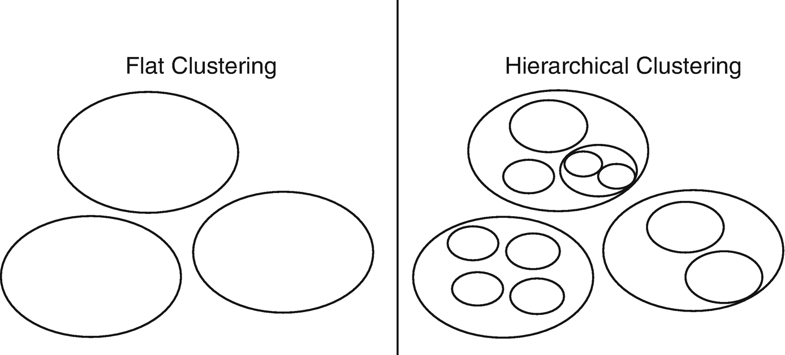
\includegraphics[scale=.4]{pic/394318_1_En_9_Fig6_HTML.png}
    \caption{扁平聚类 vs 层次聚类,核心区别是扁平聚类不体现类间关系,层次聚类反映了类的蕴含关系}
    \label{fig: cluster_taxonomy}
\end{figure}

\subsection{扁平聚类}

扁平聚类指的是得到的类,两两没有交集,所有类的并集构成了所有数据点。这一聚类的代表就是$k$-means聚类,准确说,我们先有$k$-means问题,然后才有了相关的解决这一问题的算法。$k$-means问题指的是给定数据集,寻找$k$个点使得所有点到这$k$个点的距离平方和最小。在所有解决的算法中最有名的可能就是Lloyd算法\citing{macqueen1967some}了,该算法分为以下3步。第一步,从数据集中均匀采样$k$个点作为初始化的中心点;第二步,所有点靠到离自己最近的中心点上去,形成k个类;第三步,取k个类的中心点作为新的中心点。一般来说,第二、三步会重复$t$次,因此算法的时间复杂度是$O(nkdt)$,其中$n$,$d$分别指的是待聚类的数据量和数据的维度。作为一个经典聚类算法,该算法被大量应用在自然语言处理、数据挖掘、以及其他领域中。这个算法有一些优点,首先它比较简单,易于实现。其次,它易于并行,在中等数据量下可以很好运行。但是它的一些缺点也非常瞩目,聚类的$k$值不好确定,受初始点影响大,仅能对球形数据进行聚类(如果数据非球形则聚类结果和人的直观感觉有较大出入)。

%todo: check spectral clustering
为了解决最后一个问题,谱聚类(spectral clustering)被提了出来。这一聚类算法创新性的从图分割的角度给聚类带来了新的视角,从这一视角下,一些传统上不容易被聚类的数据集也能被攻克。它的基本思想是在数据集上构建一个图,聚类问题转化为大图切割为子图的问题,好的聚类应该是,子图内部节点相似度高,子图之间相似度低。基于这一“好的”聚类的准则,人们制定了称为Ncut的切割目标函数,这一目标函数的求解可以转换为图拉普拉斯矩阵的分解问题,通过特征值分解得到新的特征,再在这一特征上聚类从而得到最终结果。
过程可总结如下:
\begin{enumerate}
    \item 根据输入的相似矩阵的生成方式构建样本的相似矩阵 $S$
    \item 根据相似矩阵 $S$ 构建邻接矩阵 $W$,构建度矩阵 $D$
    \item 计算出拉普拉斯矩阵 $L$
    \item 构建标准化后的拉普拉斯矩阵 $D^{- \frac{1}{2}}L D^{- \frac{1}{2}}$
    \item 计算 $D^{- \frac{1}{2}}L D^{- \frac{1}{2}}$最小的 $k$ 个特征值所各自对应的特征向量$f$
    \item 将各自对应的特征向量 $f$ 组成的矩阵按行标准化,最终组成 $n\times k$ 维的特征矩阵 $F$
    \item 对 $F$ 中的每一行作为一个$k$维的样本,共 $n$ 个样本,用$k$-means进行聚类,聚类数为 $k$
    \item 得到类划分
\end{enumerate}
实践中谱聚类能够很好处理$k$-means不能处理的非球形数据(比如同心圆、半月牙等),对比效果见图\ref{fig: flat_compare},这可以从谱聚类的设计准则解释,因为是做图切割,而相似度又有多种非线性的选择,所以聚类的结果就可以实现$k$-means不能做到的非线性划分($k$-means用欧式距离所以决策边界是线性的)。由于本文研究的就是$k$-means和谱聚类,所以对于他们的详细剖析见第二、三章。

\begin{figure}[h]
    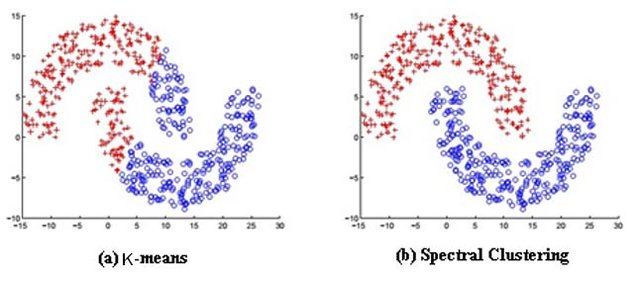
\includegraphics[scale=0.4]{pic/Comparison-between-K-Means-and-spectral-clustering_W640.jpg}
    \caption{$k$-means vs 谱聚类,可以看到谱聚类能够处理$k$-means处理不了的非球形数据}
    \label{fig: flat_compare}
\end{figure}

\subsection{层次聚类}
尽管扁平聚类的概念更简单,但我们也看到了他们的一些缺点。首先,现实世界中类和类之间是有关系的,比如说灵长类属于哺乳类,这样的蕴含关系,在扁平聚类中这样的类间关系无法体现。其次,拿$k$-means问题来说,我们需要在聚类前指定类的数目$k$,这在现实生活中未必好确定。最后,扁平聚类过程是不确定的(nondeterministic),即聚类结果有随机因素,比如Lloyd算法初始化不同结果就不同。为了解决这些问题,诞生了层次式聚类。顾名思义,层次式聚类得到的类有层级结构,可以用树状图(tree/dendrogram)来表示,如图\ref{fig: hierarchical}所示,他们也不需要指定类的数目,多数层级聚类也是确定的。这些好处的代价就是聚类速度更慢,常用的层级聚类时间复杂度至少是$O(n^2)$。

\begin{figure}[h]
    \subfloat[]{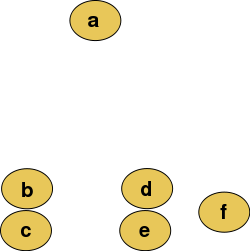
\includegraphics[scale=.5]{Clusters.svg.png}}
    \hfil
    \subfloat[]{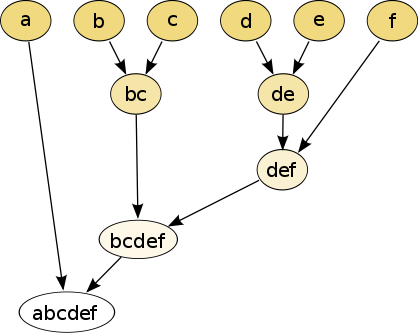
\includegraphics[scale=.4]{Hierarchical_clustering_simple_diagram.svg.png}}
    \caption{层级聚类图示。(a)示例数据集,每个字母代表一个数据点,距离越近相似度越高;(b)层级聚类后的结果,相似的类归并为一个更大的类从而形成一个二叉树,树的根节点在最下面}
    \label{fig: hierarchical}
\end{figure}

层级聚类可以自底向上做,将小的类逐渐归并得到大的类,也可以自顶向下,将大的类逐渐分割得到小的类,由此得到两种不同的聚类范式。前者称为agglomerative clustering,后者称为divisive clustering。我们先介绍前者,agglomerative clustering的一般过程如下所示
\begin{enumerate}
    \item 初始化:每个点自己作为一个类
    \item 直到所有类归并为一个类,否则
    \begin{enumerate}
        \item 找出两个最相似的类
        \item 将他们归并为一个类(父类)
    \end{enumerate}
    \item 返回类的层级结果(树)
\end{enumerate}
可以看到,这是一个贪心算法,如果有$n$个点,这个合并的过程就会持续$n-1$次,如果运气好,树的深度就是$\log_2 n$。由于树的结构,我们就可以知道类的蕴含关系,那么如何计算类和类的相似度呢?这里我们需要定义一些常用的计算方式,这些计算方式一般被称为linkage criteria,见表\ref{tab: linkage}。

\begin{table}[h]
\caption{几种常见的linkage criteria}
\begin{tabular}{cc}
\toprule
名字 & 计算方式 \\
\midrule
Maximum linkage & $\max{\{d(a,b): a \in A, b \in B\}}$ \\ 
Minimum linkage & $\min{\{d(a,b): a \in A, b \in B\}}$ \\ 
Unweighted average linkage & $\frac{1}{|A|\cdot |B|} \sum_{a \in A}\sum_{b \in B} d(a,b)$ \\
Centroid linkage & $\norm{\mu_A-\mu_B}$ \\
Ward linkage & $\frac{n_a n_b}{n_a + n_b} \norm{\mu_A-\mu_B}^2$ \\
\bottomrule
\end{tabular}
\label{tab: linkage}
\end{table}
\begin{table}[h]
\caption{几种常见的距离计算}
\begin{tabular}{cc}
\toprule
名字 & 计算方式 \\
\midrule
Euclidean distance & $\norm{a-b}_2 = \sqrt{\sum_i (a_i - b_i)^2}$ \\ 
Squared Euclidean distance & $\norm{a-b}_{2}^2 = \sum_i (a_i - b_i)^2$ \\ 
Manhattan distance & $\norm{a-b}_1 = \sum_i |a_i - b_i|$ \\
Maximum distance & $\norm{a-b}_\infty = \max_i |a_i - b_i|$ \\
\bottomrule
\end{tabular}
\label{tab: distance}
\end{table}

表格\ref{tab: linkage}中的$d$是点与点间的距离计算方式,这有很多种选择,这里挑了些常用的列在表\ref{tab: distance}中,$A,B$是两个类,$\mu_A,\mu_B$是这两个类的中心点,$n_a,n_b$是两个类中点的数目。可以看到,Maximum/Minimum/Centroid只考虑单一的点对来计算类间相似度,而Ward/Unweighted average基本考虑了全部的。值得一提的是,agglomerative clustering在聚类的过程会倾向与让大的类更大,从而导致大小不平衡的类,从这个角度讲,Minimum linkage是最差的linkage,Ward会形成差不多大小的cluster。然而在Ward中的距离计算是不可改变的(只有欧式距离),因此对于非欧的距离度量,average linkage比较合适。尽管Minimum linkage易受到噪声数据的影响,但它计算比较高效(时间复杂度是$O(n^2)$,一般的其他linkage是$O(n^2 \log n)$),因此这一linkage可以用到较大的数据量上,在非球形数据上Minimum linkage也有好的表现。

现在我们来看divisive clustering,前面说过,这是一个自顶向下的层级聚类,它需要挑选一个类,将这个类分为两个子类,并循环这个过程,直到终止条件触发(比如聚到指定数目的类)。从这个过程我们就可以看出该算法主要考虑两件事,如何挑选待分割的类以及如何分割这个类。前者一般通过某种预定义的松散度度量,比如类内最远的两个点的距离,选这个值最大的类进行分割。分割的方法一般是用扁平式聚类法,因为又包括了其他算法,divisive clustering要更复杂些。如果我们不要求划分太过细致,算法就可以在中间某层结束,如果结合Lloyd算法使用,假设我们想得到$s$个类,时间复杂度就是$O(nsdt)$,$d$和$t$分别是数据点维度和迭代次数,这样就会比agglomerative clustering快很多。有研究指出divisive clustering比 agglomerative clustering得到的层级结果质量更好\citing{karypis2000comparison},这可能是因为agglomerative是自底向上,在每次合并的时候只能看到局部的信息而不考虑全部信息,而合并过程又不可以反悔,所以divisive clustering由于是看到了全部信息做的划分,能得到更好的结果。尽管divisive clustering有这些优点,它的使用却没有agglomerative clustering频繁,可能是处理复杂情况时自底向上更符合人的习惯。

\subsection{聚类评价}
聚类评价方式分为两种,外部评价(external index)和内部评价(internal index)。前者需要有人给出的划分结果作为标准而后者不利用任何参考。我们先看外部评价,假定算法给出的类划分是$C=\{C_1, C_2,...,C_k\}$,人给出的划分是$C^* = \{C_1^*,C_2^*,...,C_s^*\}$。考虑一对数据对$(x_i,x_j)$,假设$x_i,x_j$在$C$中在同一个类里,如果算法给出的划分和人的划分是一致的,那么它们在$C^*$中也应该在同一个类里。令$\lambda_i = \{1,2,...,k\}$是数据点$x_i$的类id,即$x_i \in C_{\lambda_i}$。那么对于刚刚所说的情况可以定义一个集合$SS$来容纳这些数据对
\begin{equation*}
    SS = \{(x_i,x_j)|\lambda_i = \lambda_j,\lambda_i^* = \lambda_j^*, i<j \}
\end{equation*}
也就是说,如果数据对在$SS$集合中就意味着聚类是成功的。当然也有不成功的情况,我们定义为$SD$和$DS$。
\begin{gather*}
    SD = \{(x_i,x_j)|\lambda_i = \lambda_j,\lambda_i^* \neq \lambda_j^*, i<j \} \\
    DS = \{(x_i,x_j)|\lambda_i \neq \lambda_j,\lambda_i^* = \lambda_j^*, i<j \} \\
    DD = \{(x_i,x_j)|\lambda_i \neq \lambda_j,\lambda_i^* \neq \lambda_j^*, i<j \}
\end{gather*}
最后一行是另外一种成功的情况称为$DD$。值得注意的是,这几种情况是互不相交的,定义
\begin{equation*}
    TP = |SS|, FP = |SD|, FN = |DS|, TN = |DD|
\end{equation*}
因此有$TP+FP+FN+TN=n(n-1)/2$。基于$TP$、$FP$、$FN$和$TN$,我们可以定义以下外部评价指标($F_1$,Rand系数,Jaccard系数)
\begin{gather*}
    P = \frac{TP}{TP+FP},R = \frac{TP}{TP+FN}, F_1 = \frac{2*P*R}{P+R} \\
    \text{Rand} = \frac{TP+TN}{TP+FP+FN+TN} \\ 
    \text{Jaccard} = \frac{TP}{TP+FP+FN}
\end{gather*}
$F_1$和监督学习中的一致,Rand系数也被称为Accuracy。除去上面这些还有简单实用的Purity以及有信息论背景的NMI(Normalized Mutual Information),当类的数目比较大的时候,Purity容易比较大,而NMI缓解了此问题。
\begin{gather*}
    \text{Purity} = \frac{1}{n} \sum_i \max_j n_{ij} \\
    \text{MI}(C, C^*) = \sum_{i=1}^{|C|}\sum_{j=1}^{|C^*|}P(i, j)\log\left(\frac{P(i,j)}{P(i)P(j)}\right) \\
    H(C) = - \sum_{i=1}^{|C|}P(i)\log(P(i)) \\
    \text{NMI}(C, C^*) = \frac{\text{MI}(C, C^*)}{\text{mean}(H(C), H(C^*))}
\end{gather*}

其中,$n_{ij}=|C_i \cap C_j^*|$,$n_i = |C_i|$,$P(i) = n_i/n$,$P(i,j)=n_{ij}/n$。$P(i)$可以理解为一个数据点落在类$i$中的概率,$P(i,j)$可以理解为一个点在既在$C_i$又在$C_j^*$中的概率。MI称为互信息(mutual information),H是熵。这里所列的外部评价都是越大越好。

除了外部评价,内部评价在没有人工标注的情况下使用,比如$k$-means的目标值(objective)可以作为评价指标,该评价指标是聚类问题相关的,评价$k$-means算法用,评价其他算法慎用,还有一些聚类问题无关的评价指标,比如DB指数(Davies-Bouldin Index)
\begin{gather*}
    \text{avg} = \frac{2}{|C|(|C|-1)}\sum_{1\leq i<j \leq |C| }d(x_i,x_j) \\
    d_{cen}(C_i,C_j) = d(\mu_i,\mu_j) \\
    \text{DBI} = \frac{1}{k}\sum_{i=1}^k \max_{j \neq i} (\frac{\text{avg}(C_i)+\text{avg}(C_j)}{d_{cen}(\mu_i,\mu_j)})
\end{gather*}
其中$d$可以是表\ref{tab: distance}中的距离函数。

\section{本文的研究目标及主要贡献和创新}
在大数据下聚类,我们应该关心什么问题呢?我们应该注意那些普遍且真实的问题,所以,首先,我们应该考虑的就是聚类速度,传统聚类算法由于其自身较高的时间复杂度,在目前大数据时代越来越难以适用。其次,聚类算法的聚类质量也是一个主要问题,很多算法声称自己有好的聚类质量,并且也在一部分数据上得到了证实,但是可能换一个数据集这个算法效果就不好了,对于这种情况有时很难分析问题在哪里,这种时候我们就会希望这个算法在理论上有质量保证,比如说可以证明该算法不会比最优算法的聚类结果差多少倍。总结一下,在本文中我们将探究以下两个问题:
\begin{enumerate}
    \item 怎样聚类更加高效?
    \item 怎样聚类得出的解有理论保证?
\end{enumerate}
鉴于扁平聚类的普适性,我们将围绕$k$-means问题和谱聚类问题探究我们所提出的问题并给出我们的贡献。具体来说,我们的贡献和创新有以下几点:
\begin{enumerate}
    \item (理论\&实验贡献)对基于均匀采样加速$k$-means的算法给出了更紧的理论界,从$4(\alpha+\beta)$收缩到了$\alpha+\beta$,同时,我们证明了在温和的假设下,该算法的时间复杂度在多项式对数级别(polylogarithmic time),随后我们在实验上对理论结果进行了验证
    \item (理论贡献)将经典的$k$-means++初始化方法扩展到了带权重的$k$-means问题上并给出了证明
    \item (理论\&实验贡献)对基于Weighted kernel $k$-means的谱聚类算法给出了更紧的理论界,并给出了Weighted kernel $k$-means的MATLAB实现。
\end{enumerate}

\section{本论文的结构安排}
本文的章节结构安排如下:第一章是绪论,介绍常见聚类算法为后续探讨打下初步基础同时明确指出要研究的问题和我们的创新,第二章探讨$k$-means问题,将会分别深入分析与回答我们所提出的两个问题。第三章探讨谱聚类问题,同样加速和理论保证分别分析。第四章是结论,在总结全文的基础上给出未来可能的研究方向。